\documentclass{article}[letterpaper, margins=1in, 12pt]
\usepackage[a4paper,bindingoffset=0.2in,%
            left=1in,right=1in,top=1in,bottom=1in,%
            footskip=.25in]{geometry}
\usepackage{authblk}
\usepackage{amsmath}
\usepackage{listings}
\usepackage{graphicx}
\usepackage{wrapfig}
\usepackage[maxbibnames=99]{biblatex}
\addbibresource{REU_report.bib}
\graphicspath{{./images/}}
\usepackage{xcolor}

\definecolor{codegreen}{rgb}{0,0.6,0}
\definecolor{codegray}{rgb}{0.5,0.5,0.5}
\definecolor{codepurple}{rgb}{0.58,0,0.82}
\definecolor{backcolour}{rgb}{0.95,0.95,0.92}

\lstdefinestyle{mystyle}{
    backgroundcolor=\color{backcolour},   
    commentstyle=\color{codegreen},
    keywordstyle=\color{magenta},
    numberstyle=\tiny\color{codegray},
    stringstyle=\color{codepurple},
    basicstyle=\ttfamily\footnotesize,
    breakatwhitespace=true,         
    breaklines=true,                 
    captionpos=b,                    
    keepspaces=true,                 
    numbers=left,                    
    numbersep=5pt,                  
    showspaces=false,                
    showstringspaces=false,
    showtabs=false,                  
    tabsize=2
}

\lstset{style=mystyle}

\title{Technical Report: SPIDAL Summer REU 2021 Upgrading MDPOW and Adding Analysis Functionality}
\date{\today}
\author{Alia Lescoulie}
\affil{Department of Chemistry and Biochemistry, College of Science and Mathematics, California Polytechnic State University, San Luis Obispo, CA, 93407}

\begin{document}
\maketitle

\begin{abstract}
MDPOW is an open source Python package for calculating water-octanol and water-cyclohexane partition coefficients using the molecular dynamics package GROMACS. During the SPIDAL REU, MDPOW was updated to support Python 3. A collection of classes were constructed, to simplify development of simulation analyses. These objects were designed for efficient and organized storage of a group of molecular dynamics systems, and provide a basic framework for developing analyses. All code is included in the latest release of MDPOW at https://github.com/becksteinlab/mdpow.
\end{abstract}

\section{Introduction}
Molecular dynamics (MD) is one method for computing water-octanol partition coefficients ($P_{ow}$) of drug-like molecules. This is accomplished through calculating the free energy of solvation from the simulation. With free energy values from water and octanol the partition coefficient can be obtained using $P_{ow} = {(\Delta G_w - \Delta G_o)}/{(RT)} \log(e)$ where $R=8.31446261815 \times 10^{-3} \: \text{{kJ}}/{ \text{mol} \cdot \text{K}}$ is the universal gas constant and $e$ is Euler's number \cite{fan_precise_2021}.

A number of methods exist for obtaining free energies of systems in MD simulations. The two discussed here are Bennett Acceptance Ratio (BAR) and Thermodynamic Integration (TI) \cite{pohorille_good_2010}. The free energy change $\Delta A$ from the canonical partition function $Q$ is defined by the following \cite{chipot_free_2007}:

\begin{equation}
\Delta A = - \frac{\ln{Q_1 / Q_0}}{\beta}
\end{equation}

BAR overcomes the challenge of calculating partition functions by substituting the ratio of the partition functions $Q_1 / Q_0$ for the ratio of probabilities ($M_0 / M_1$) for a trial move which maintains the same configurational space but switches potential energies from the reference system $U_0$ to the unknown system $U_1$ and vice-versa \cite{bennett_efficient_1976}. The potential energy can be calculated with system positions.

Thermodynamic integration (TI) obtains changes in free energy by defining a parameter $\lambda$ such that at $\lambda = 0 \; U = U_0$ and at $\lambda = 1 \; U = U_1$, where $U_1$ is the final state and $U_0$ is the initial state, and taking the partial derivative of $A$ with respect to $\lambda$ and integrating from 0 to 1 \cite{chipot_free_2007}.

Both BAR and TI use $\lambda$ as a parameter for the extent of solute-solvent interactions \cite{chipot_free_2007}. This requires running a MD simulation for  each interaction at their respective $\lambda$ values \cite{lemkul_proteins_2019}. The process of initializing that number of simulations requires either the creation of a shell script running each or a tedious process of manually navigating directories, copying files, and running simulations. MDPOW makes this process easier with the user simply defining their settings and supplying a coordinate file, then running a few Python scripts.

MDPOW is not without its limitations. Before release 0.7.0 it was incompatible with anything newer than Python 2.7 and had few features for analysis beyond running BAR and TI calculations. Both of these features were added over the course of the SPIDAL REU.

Incompatibility with Python 3 created a number of challenges, in particular compatibility with newer versions of dependencies such as MDAnalysis, which dropped Python 2 compatibility \cite{michaud-agrawal_mdanalysis_2011, gowers_mdanalysis_2016}. This made new development more difficult, and meant that users had to create an environment for MDPOW separate from the environment used for other portions of a project. For version 0.7.0, retaining Python 2 cross-compatibility was  necessary due to the long-term nature of scientific projects. This meant that many of the new features added in Python 3 such as f-strings, and in Python 3.6 and later, type annotations, were unavailable during the update process \cite{fan_precise_2021, beckstein_prediction_2012}.

\begin{wrapfigure}{r}{0.25\textwidth}
	\centering
	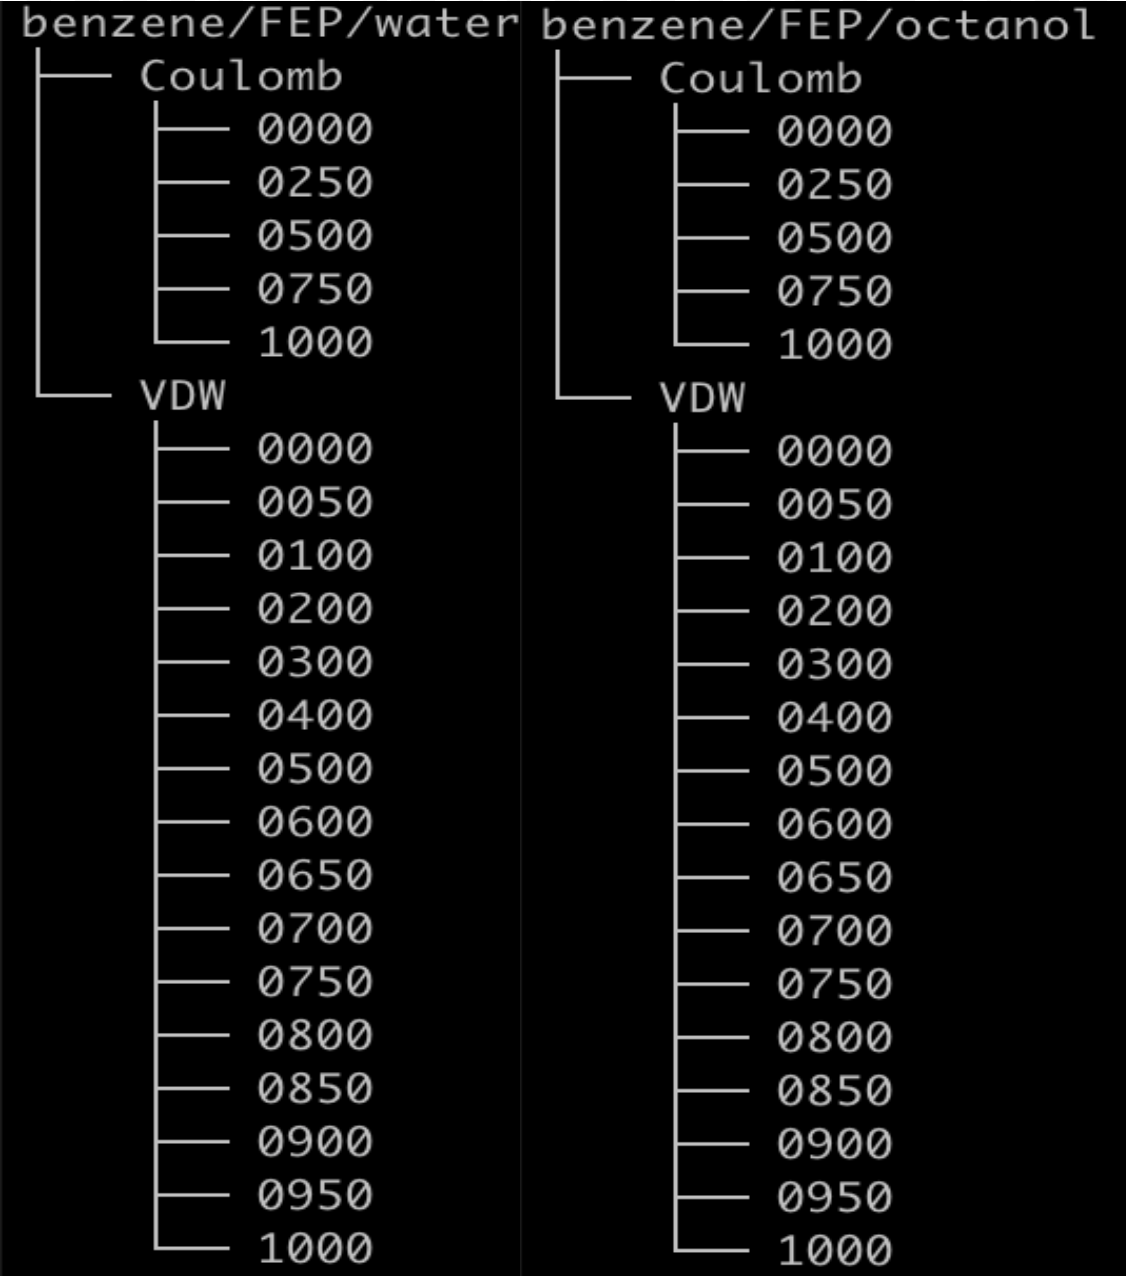
\includegraphics[width=0.25\textwidth]{directory}
	\caption{Example MDPOW FEP directory structure}
	\label{fig:directory}
\end{wrapfigure}

An additional shortcoming of MDPOW addressed during the REU was its lack of a simple methodology for analyzing sets of alchemical free energy simulations. MDPOW, when running free energy perturbation (FEP) simulations, establishes a directory like the example in Fig \ref{fig:directory}, with simulation files sorted by solvent, interaction and $\lambda$-value. Running a simulation to get the partition coefficient can result in forty or more individual systems. For example using MDAnalysis \texttt{Universe} objects to load systems, one would have to write code to individually load each simulation each in its own directory. That's not to mention actually running analyses on that set of systems. Requiring users to each develop their own analysis tools for managing a larger number of systems would result in lost time and repeated work. Providing an analysis framework makes the process more user friendly.

\section{Methods}
\subsection{Modernizing MDPOW}

The differences between Python 2 and Python 3 presented compatibility issues in a number of key areas primarily: outdated tests, pickle compatibility issues, and changes to syntax. The first issue was ensuring that all tests ran in both Python versions so that cross compatibility could be validated. MDPOW testing is done in pytest, which eliminated yield tests in version 4.0 requiring their replacement. This was done using parameterization tests where the test parameter and a list of inputs are provided to a function. In the process of running tests, it became apparent reading pickle files was an incompatibility between versions. Pickle files, which save an instance of a Python object as a file, are used throughout MDPOW, particularly in testing. Pickles encoded in Python 2.7, when read normally using the six library in Python 3 raised byte errors. To solve this, pickle loading code was replaced with the block below throughout MDPOW. 

\begin{lstlisting}[language=Python]
if sys.version_info.major >= 3:
	with open(gsolv, 'rb') as f:
		G = pickle.load(f, encoding='latin1')
elif sys.version_info.major == 2:
	G = pickle.load(gsolv.open())
\end{lstlisting}

By checking for the version, pickles can be loaded in byte mode when code is run in Python 3, ensuring compatibility. Patches like this, where separate blocks of code are executed based on version were avoided, but in this case was unavoidable. In MDPOW version 0.8.0 Python 2 support was dropped, and this style of patch has been replaced. The tests and pickle file represented the bulk of compatibility issues. Aside from that the remaining issues were simply the result of syntax differences present in older version of Python.

\subsection{Implementation of Analysis Features}

Addressing the aforementioned challenge of managing several simulations the \texttt{Ensemble} object was developed. The \texttt{Ensemble} object is a collection of MDAnalysis \texttt{Universe}s stored in a Python dictionary. Python dictionaries, a type of hash table, have O(1) average search efficiency. This means that the time required to find an item is independent of the size of the table \cite{cormen_introduction_2009}. This search efficiency, and the organization created by the key-value pair structure of dictionaries, were the reasons for their selection when developing the \texttt{Ensemble} object. An \texttt{Ensemble} object is able to load the trajectory files present in a MDPOW molecules directory, automatically handling the process of  directory navigation and system loading.  The \texttt{Ensemble} object also replicates some of the functionality present in MDAnalysis \texttt{Universe} objects, namely it allows users to select atoms from the systems it stores. This returns a \texttt{EnsembleAtomGroup}  object.

The \texttt{EnsembleAtomGroup}  is to the MDAnalysis AtomGroup as the \texttt{Ensemble} is to the MDAnalysis \texttt{Universe}. It is initialized by the select atoms command of Ensemble. It, like the \texttt{Ensemble} attempts to extend the functionality of MDAnalysis objects to collections of those objects. It has class methods to select atoms, return positions, and return the original \texttt{Ensemble} object. The code example below shows how an \texttt{Ensemble} can be initialized from a simulation directory, and how an \texttt{EnsembleAtomGroup} is created from an \texttt{Ensemble}.

\begin{lstlisting}[language=Python]
benzene_dir = os.path.join('mdpow', 'tests', 'testing_resources',
													 'states', 'benzene')
Benzene = mdpow.ensemble.Ensemble(dirname=benzene_dir)
DihedralGroup = Benzene.select_atoms('name C1 or name C2 or name C3 or name C4')
\end{lstlisting}

With the \texttt{Ensemble} and \texttt{EnsembleAtomGroup} objects an analysis framework analogous to AnalysisBase in MDAnalysis was developed for running calculations on collection of systems generated by MDPOW. Setting up an analysis for a MDPOW simulation requires simply sub classing \texttt{EnsembleAnalysis} as in the next listing. To implement an analysis, an \texttt{EnsembleAnalysisBase} subclass with a few basic methods must be defined. For an analysis to work it needs an \lstinline{__init__} to accept parameters, a \lstinline{_prepare} to create a place to store data, a \lstinline{_single_universe} or \lstinline{_single_frame} that runs an analysis generating data. A more detailed explanation of designing an analysis can be found in section 3.1.1.

\begin{lstlisting}[language=Python]
class ExampleAnalysis(mdpow.ensemble.EnsembleAnalysis):
	def __init__(self, ExampleEnsemble):
		super(ExampleAnalysis, self).__init__(ExampleEnsemble.ensemble())
		self._ensemble = ExampleEnsemble

	def _prepare_ensemble(self):
		self._cols = ['solvent', 'interaction', 'lambda', 'time', 'result']
		self._result_dict = {x: [] for x in self._cols}
		self.results = pd.DataFrame(column=self._cols

	def _single_frame(self):
		result = analysis_function(self._ensemble[self._key])
		res_list = [self._key[0], self._key[1], self._key[2], self._ts.time, result]
		for i in range(len(res_list)):
			self._result_dict[self._col[i]].append(self.res_list[i])

	def _conclude_ensemble(self):
		for k in self._result_dict:
			self.results[k] = self._result_dict[k]

\end{lstlisting}

\texttt{EnsembleAnalysis} was developed to be similar to AnalysisBase in MDAnalysis. When developing an analysis several aspects must be defined; an \lstinline{__init__}, which accepts parameters in this case lines 2-4. Among the parameters must be at least one Ensemble, which must be passed back to the parent class using the \lstinline{super} function from Python as seen in line 3. Next \lstinline{_prepare_ensemble} and \lstinline{_prepare_universe} can be used to establish data structures used in the overall analysis and the individual systems. In lines 6-9 on the example a results dictionary and \texttt{DataFrame} are set up for organizing results by solvent, interaction, lambda, and time. Next are the methods responsible for generating results from the MD simulations, \lstinline{_single_universe} which runs on each system in the \texttt{Ensemble}, and \lstinline{_single_frame} which runs on each frame of each \texttt{Universe}. \lstinline{_conclude_universe} and \lstinline{_conclude_ensemble} are run after each \texttt{Universe} and the \texttt{Ensemble} respectively. When an \texttt{EnsembleAnalysis} based object is run, each system stored in the provided \texttt{Ensemble} is iterated over with \lstinline{_single_universe} ran at that point, and \lstinline{_single_frame} run on each frame of the \texttt{Universe}. In this case \lstinline{_single_frame} consists of an example \lstinline{example_function} which returns a result on line 12. In the proceeding lines that result is stored in \lstinline{_result_dict} which was created in \lstinline{_prepare_ensemble}. All of the information from each frame is recorded to ensure that the data is "tidy"\cite{tidy-data}. Afterwards there is the option to define \lstinline{_conclude_universe} which runs each time a new system is completed allowing for processing to occur after each system. Finally after iteration is complete \lstinline{_conclude_ensemble} is run. In this case it saves the contents of the results dictionary into the results \texttt{DataFrame}, this is done at the end because dictionaries are far simpler to add data to within the program, but \texttt{DataFrame} is more convenient for saving and plotting data. In the final \texttt{DataFrame} each index has a all the information, 'solvent', 'interaction', 'lambda', 'time', and 'result'. This allows for easy organization of data by multiple parameters for example returning all the results for water and VDW.

\section{Results and Discussion}

With the establishment of a framework for analyzing collections of simulations, such as those generated by FEP calculations, the process of developing analyses for MDPOW simulations is simplified. These are developed using objects created as subclasses of \texttt{EnsembleAnalysis}.

\subsection{Implemented EnsembleAnalysis Methods}
Using the \texttt{EnsembleAnalsis} framework two new methods were developed as part of the new MDPOW analysis submodule. The first to be discussed is \texttt{SolvationAnalysis} which quantifies solvent molecules within the given cutoff distances. It is discussed in section 3.2.1 specifically focusing on how to design an \texttt{EnsembleAnalysis} based class. The second is \texttt{DihedralAnalysis} in section 3.2.2 which discusses considerations for efficient design of \texttt{EnsembleAnalysis} classes.

\subsubsection{Solvation Shell: Example for the EnsembleAnalysis Framework}

One of the analyses developed with the \texttt{EnsembleAnalysis} framework, \texttt{SolvationAnalysis}, which returns the number of solvents within the given distances, can also serve as an example of how to develop an analysis more generally. 

\texttt{SolvationAnalysis} quantifies the number of solvent atom within a given distance of the solute. It accomplishes this through calculating the distances between and each molecule using the \lstinline{capped_distance} function from MDAnalysis to get the indices for pairs which fall within the given cutoff \cite{michaud-agrawal_mdanalysis_2011, gowers_mdanalysis_2016}. 

Building \texttt{EnsembleAnalysis} using inheritance, a concept from object oriented programming, simplifies the process of programming an analysis. Inheriting from a superclass gives a subclass the same methods and attributes, meaning that some methods common to all \texttt{EnsembleAnalysis} objects like \lstinline{run} can be retained; other methods the user can override to run their own analysis code. To develop \texttt{SolvationAnalysis}, only three methods were overridden in the subclass.  
 
\begin{lstlisting}[language=Python]
class SolvationAnalysis(EnsembleAnalysis):
       def __init__(self, solute: EnsembleAtomGroup, solvent: EnsembleAtomGroup, distances: List[float]):
        self.check_groups_from_common_ensemble([solute, solvent])
        super(SolvationAnalysis, self).__init__(solute.ensemble)
        self._solute = solute
        self._solvent = solvent
        self._dists = distances

    def _prepare_ensemble(self):
        self._col = ['distance', 'solvent', 'interaction',
                     'lambda', 'time', 'N_solvent']
        self.results = pd.DataFrame(columns=self._col)
        self._res_dict = {key: [] for key in self._col}

    def _single_frame(self):
        solute = self._solute[self._key]
        solvent = self._solvent[self._key]
        pairs, distances = capped_distance(solute.positions, solvent.positions,
                                          max(self._dists), box=self._ts.dimensions)
        solute_i, solvent_j = np.transpose(pairs)
        for d in self._dists:
            close_solv_atoms = solvent[solvent_j[distances < d]]
            result = [d, self._key[0], self._key[1],self._key[2],
                      self._ts.time, close_solv_atoms.n_atoms]
            for i in range(len(self._col)):
                self._res_dict[self._col[i]].append(result[i])

    def _conclude_ensemble(self):
        for k in self._col:
            self.results[k] = self._res_dict[k]
\end{lstlisting}

The first method \lstinline{__init__} accepts arguments needed to generate an instance of the object. In this case the user selected solute and solvent, contained in \texttt{EnsembleAtomGroup}s, and a list of the distances to be measured. On line 2 the \lstinline{__init__} ensures that the two \texttt{EnsembleAtomGroup} objects originate from the same \texttt{Universe} using a built in method of \texttt{EnsembleAnalysis} called \lstinline{check_groups_from_common_ensemble}. This is important as the the groups in \lstinline{_single_frame} must both exist in the same \texttt{Universe}. Next the \texttt{Ensemble} from the aforementioned groups is passed into the parent class with the \lstinline{super} function in line 4. Finally the items are saved as class attributes (saved in the class, and accessible to other methods). The underscore in front of method and attribute names by Python convention indicates that it is protected.

The next method \lstinline{_prepare_ensemble} establishes data structures needed in the analysis. The final results are available to the user in a \texttt{DataFrame}, but for the sake of efficiency the results are stored in arrays contained in a dictionary with the same keys as the columns in the \texttt{DataFrame} as the analysis is run. On line 13 for brevity dictionary interpretation is give each key a blank array.  With structures established for storing the results the next methods can focus on obtaining information from the simulation.

\begin{wrapfigure}{r}{0.25\textwidth}
	\centering
	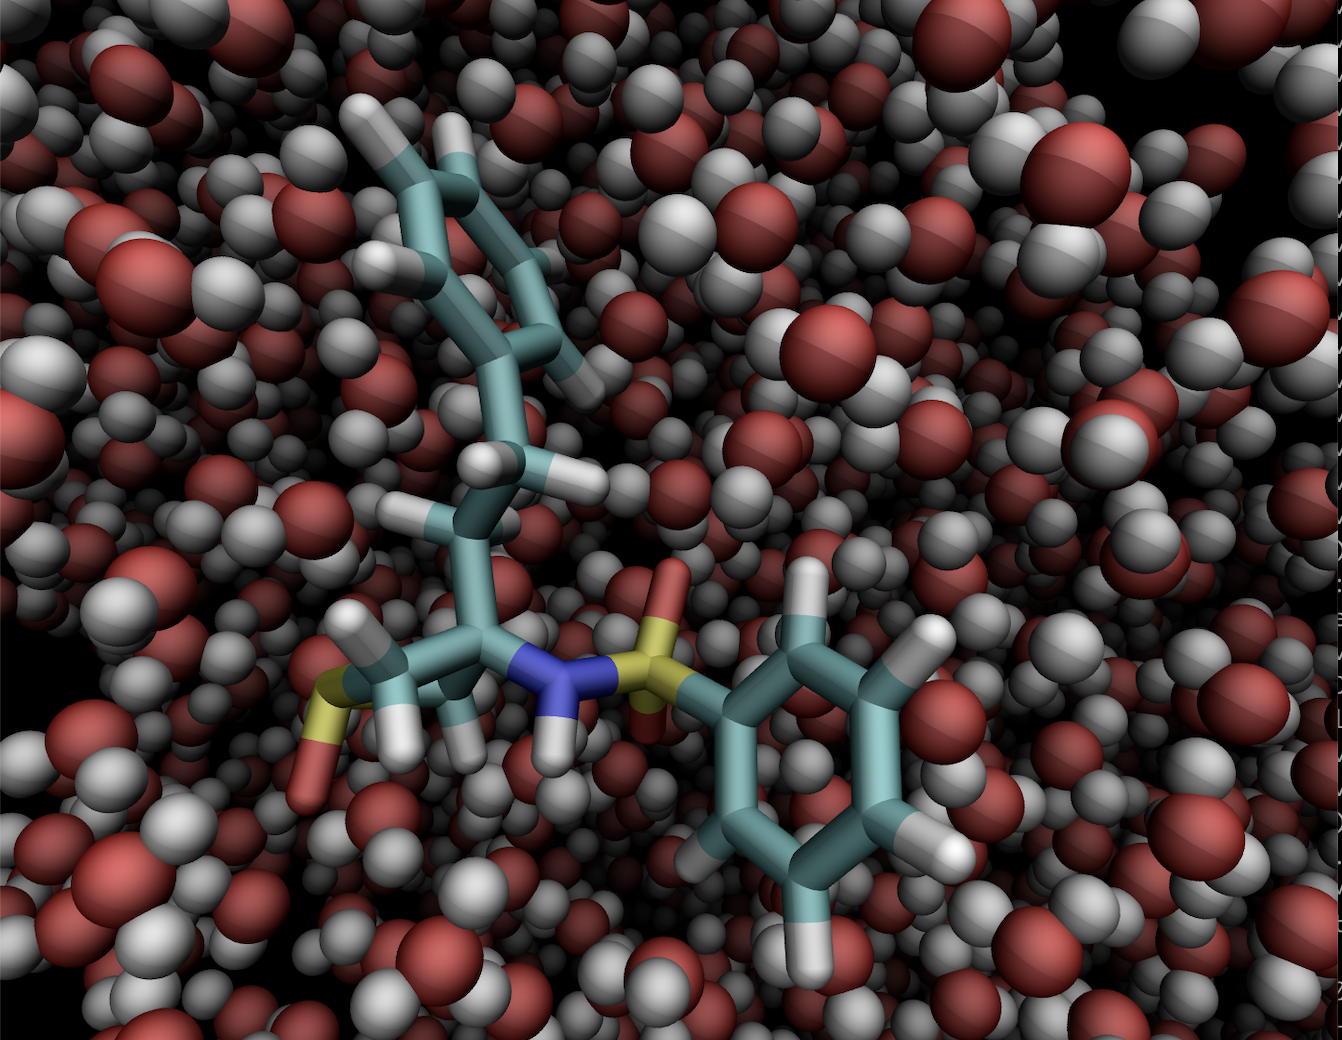
\includegraphics[width=0.25\textwidth]{solvent}
	\caption{Solute in surounded by water molecules.}
	\label{fig:solute}
\end{wrapfigure}

With data structures lined up, the actual number of solvent molecules can be counted with \lstinline{_single_frame}. This is done using the fast capped distances function in MDAnalysis on line 18. This computes a distance array for the given group positions and returns distances in that range \cite{michaud-agrawal_mdanalysis_2011, gowers_mdanalysis_2016}.

Finally the \lstinline{_res_dict} data is inputted into the results DataFrame. This gives data that is neatly organized and easy to generate figures from. The data obtained from \texttt{SolvationShell} gives an idea of how solvent molecules are distributed around the solute. This data can also be compared between different $\lambda$ values in a alchemical free energy simulation, offering incite into the role of different intermolecular interactions in the solvation process.

This analysis was developed to determine arrangement of solvents around the solute. Figure 2 is SM36 from the SAMPL7 data set shows a rendering of the solute sew rounded by water molecules \cite{fan_precise_2021}. \texttt{SolvationAnalysis} works by counting the solvents within the given cutoff's. The relationship between distance and number of solvent molecules for the solvent in figure 2 is shown in figure 3. The collected data sorted with Coulomb on the left and VDW on the right shows that the solvent molecules arrangement around the solute is dependent on their interactions.

\begin{figure}[h]
    \centering
	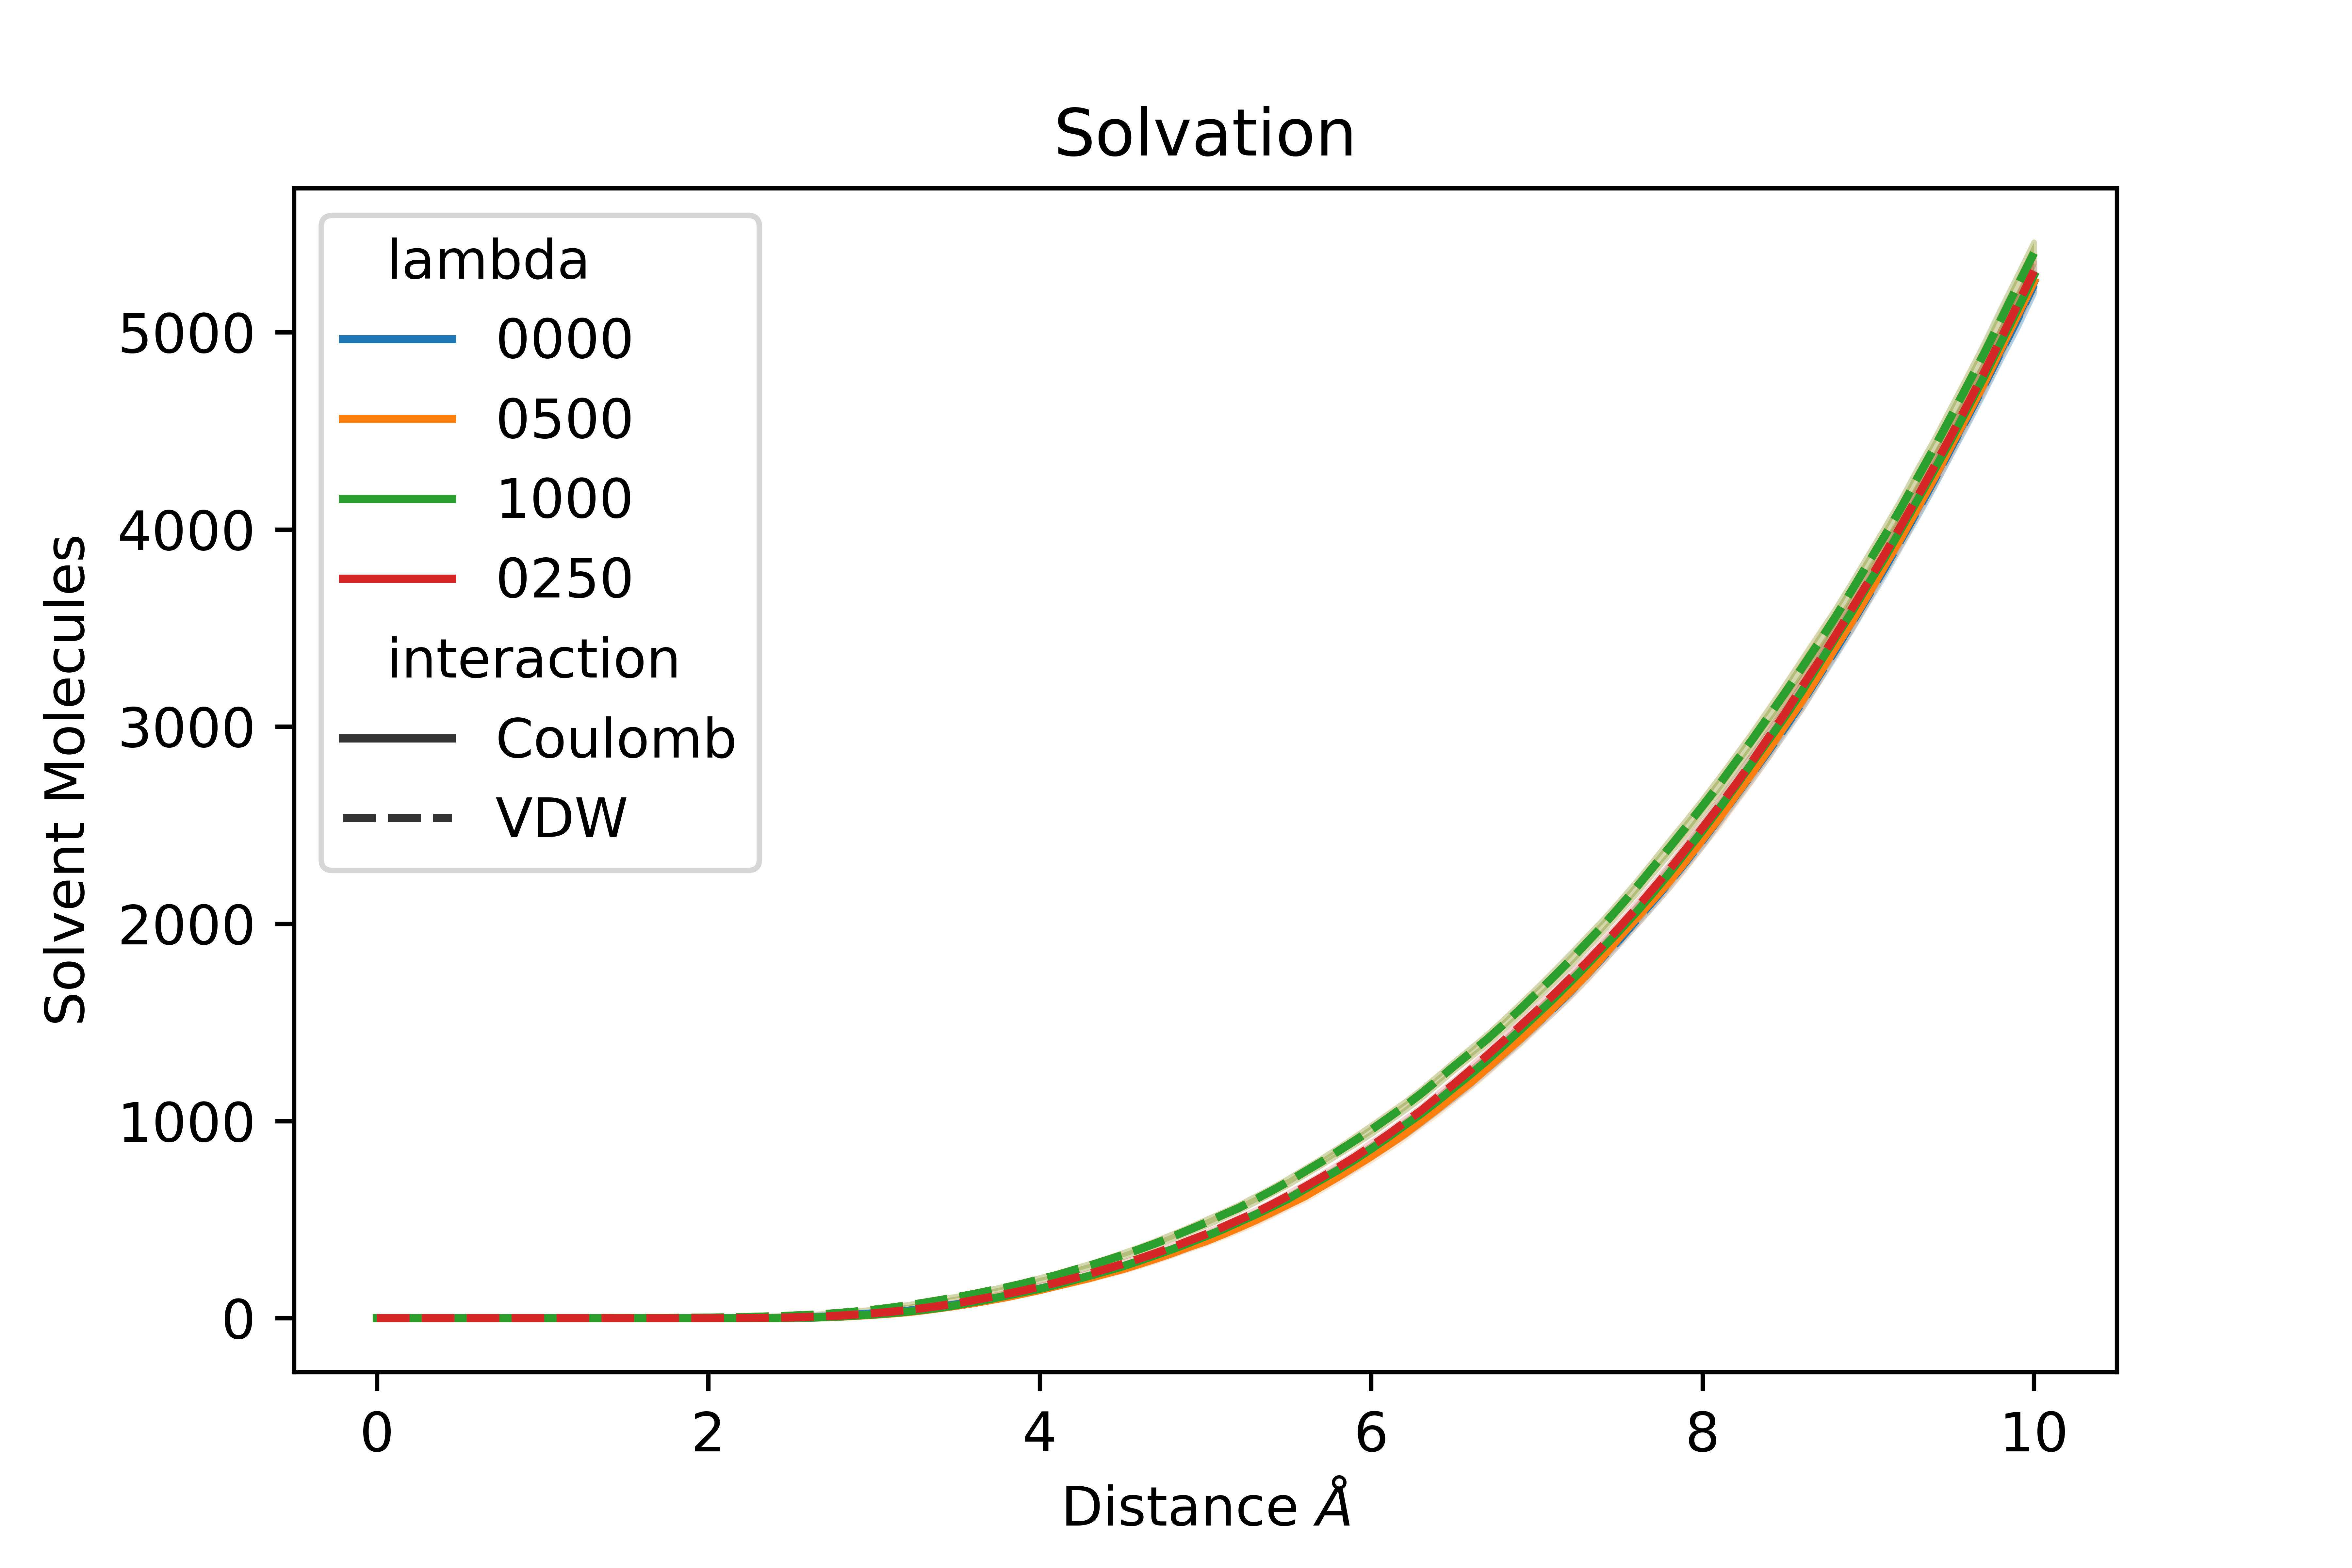
\includegraphics[scale=0.5]{solv_plot}
	\caption{Example solvation shell plot}
	\label{fig:solvation}
\end{figure}
 

\subsubsection{Dihedral Analysis: Building an EnsembleAnalysis Efficiently}

Additionally \texttt{DihedralAnalysis} was developed using the \texttt{EnsembleAnalysis} framework. \texttt{DihedralAnalysis} accepts a list of \texttt{EnsembleAtomGroup} objects and returns the dihedral angles over the course of the trajectory. It accomplishes this using the \lstinline{calc_dihedrals} function from MDAnalysis \cite{michaud-agrawal_mdanalysis_2011, gowers_mdanalysis_2016}. This function is written in Cython, which translates python code to C, making it significantly faster than code written in python \cite{Mull2018}. 

\begin{figure}[h]
    \centering
	\includegraphics[scale=0.5]{Dihedral}
	\caption{\textbf{A.} Dihedral C-N-S-C (1 - 2 - 3 - 4) from SM36. \textbf{B.} Plot of execution time for repackaging method (top) and iterating (bottom).} 
	\label{fig:dihedral}
\end{figure}

Dihedral angles are calculated from the positions of four atoms, and describe the geometry of two portions of a molecule between a chemical bond. This gives a better understanding of the spatial relationship between groups in a molecule. Figure 4.A demonstrates how a dihedral can quantify the arrangment of larger groups in a molecul, in that case the orientation of the phenyl group on the carbon labeled 4 relative to benzyl group on the carbon labeled 1. 

Two different implimentations were tested during the development of \texttt{DihedralAnalysis}, itterative and The implementation of \texttt{DihedralAnalysis} in MDPOW was based on the MDAnalysis version designed for one \texttt{Universe}, accepting a list of \texttt{AtomGroup} objects each containing the four atoms of a dihedral group. It then repackages that list of \texttt{AtomGroup} objects into four groups each containing one atom from the user given list \cite{Mull2018}. The advantage of this approach is that for each frame of the trajectory \lstinline{calc_dihedrals}, which can accept arrays, is only run a single time, calculating the list of dihedrals simultaneously. This is more efficiency due to the aforementioned efficiency of code run in C as compared to python.

\texttt{DihedralAnalysis} replicated this approach, but extended it to a list of \texttt{EnsembleAtomGroup}. Prior to running calculations, the dihedral group atoms are repacked into new \texttt{AtomGroup}s each containing one atom from each provided dihedral group. Those \texttt{AtomGroup}s are then repackaged into four \texttt{EnsembleAtomGroup}s, ensuring that, like in the MDAnalysis version, \lstinline{calc_dihedrals} is only called once per trajectory frame rather than repeataly as the list of dihedrals is itterated over.
 
When applied to \texttt{EnsembleAtomGroup}s the added inefficiency of repackaging the dihedral groups outweighed the added efficiency of removing iteration from \lstinline{_single_frame}. This was found by comparing the execution time of the two methods as additional dihedral groups were added as seen in figure 4.B. The iterative method outperformed the repackaging method by a relatively consistent margin each time. 

\section{Conclusion}
The modernization of MDPOW and development of the analysis submodule over the course of the SIPDAL REU increased the usability and utility of the library. The update to Python 3 will ensure compatibility with future versions of dependency libraries, and ensure access to future features of those libraries. Additionally the \texttt{Ensemble} objects and \texttt{EnsembleAnalysis} framework simplify the development of analytical tools within MDPOW.

\section*{Acknowledgments}
Funding was provided by the National Science Foundation for a REU supplement to award ACI1443054. 

\printbibliography
\end{document}

